\documentclass{standalone}

% font set
\usepackage{ctex}
\usepackage{fontspec}
\usepackage[sc]{mathpazo}
\usepackage{anyfontsize}

\setmainfont{SourceSerif4-Regular.ttf}[%
    Path = ../../fonts/,
    BoldFont = SourceSerif4-Bold.ttf,
    ItalicFont = SourceSerif4-It.ttf,
    BoldItalicFont = SourceSerif4-BoldIt.ttf
]
\setCJKmainfont[%
    Path = ../../fonts/,
    BoldFont=SourceHanSansSC-Medium.otf,
    ItalicFont=gkai00mp-2.ttf%
]{SourceHanSansSC-Normal.otf}

% colors
\usepackage[dvipsnames]{xcolor}
\definecolor{pku-red}{RGB}{139,0,18}
\usepackage{colortbl}
\newcommand{\light}[1]{\textcolor{Orchid}{#1}}
\newcommand{\contrastlight}[1]{\textcolor{TealBlue}{#1}}

\usepackage[normalem]{ulem}

\usepackage{makecell}

% math package
\let\Bbbk\relax
\usepackage{amsmath}
\usepackage{mathrsfs}
\usepackage{amssymb}
\usepackage{amsfonts}
\usepackage{stmaryrd}
\usepackage{latexsym}
\usepackage{extarrows}
\SetSymbolFont{stmry}{bold}{U}{stmry}{m}{n}
\allowdisplaybreaks[3]


% math notations
\newcommand{\LHS}{\mathrm{LHS}}
\newcommand{\RHS}{\mathrm{RHS}}
\newcommand{\Z}{\mathbb{Z}}
\newcommand{\N}{\mathbb{N}}
\newcommand{\R}{\mathbb{R}}
\newcommand{\Q}{\mathbb{Q}}
\newcommand{\C}{\mathbb{C}}
\newcommand{\E}{\mathbb{E}}
\renewcommand{\O}{\mathcal{O}}
\newcommand{\id}{\mathrm{id}}
\DeclareMathOperator*{\Span}{Span}
\DeclareMathOperator*{\im}{Im}
\DeclareMathOperator*{\rank}{rank}
\DeclareMathOperator*{\card}{card}
\DeclareMathOperator*{\grad}{grad}
\DeclareMathOperator*{\argmax}{argmax}
\DeclareMathOperator*{\epi}{epi}
\DeclareMathOperator*{\maximize}{maximize}
\DeclareMathOperator*{\minimize}{minimize}
\renewcommand{\d}{\mathrm{d}}
\newcommand{\Pow}{\mathcal{P}}
\newcommand{\cov}{\mathsf{Cov}}
\newcommand{\var}{\mathsf{Var}}
\newcommand{\Nor}{\mathcal{N}}
\newcommand{\U}{\mathcal{U}}
\renewcommand{\t}{\mathsf{T}}
\newcommand{\T}{\top}
\newcommand{\F}{\bot}
\newcommand{\norm}[1]{\left\|#1\right\|}
\newcommand{\inner}[2]{\left\langle{#1},{#2}\right\rangle}
\newcommand{\e}{\mathrm{e}}
\newcommand{\const}{\mathrm{const}}
\newcommand{\scB}{\mathscr{B}}
\newcommand{\scF}{\mathscr{F}}
\newcommand{\G}{\mathscr{G}}
\newcommand{\Exp}{\mathsf{Exp}}
\newcommand{\DExp}{\mathsf{DExp}}
\newcommand{\Lap}{\mathsf{Lap}}
\newcommand{\calP}{\mathcal P}
\newcommand{\calS}{\mathcal S}
\newcommand{\calF}{\mathcal F}
\newcommand{\calM}{\mathcal M}
\newcommand{\KL}{\mathrm{KL}}
\newcommand{\ReLU}{\mathsf{ReLU}}
\newcommand{\val}{\mathsf{val}}

% plots
\usepackage{tikz}
\usetikzlibrary{arrows}
\usetikzlibrary{arrows.meta,positioning,calc,3d,fit}
\usetikzlibrary{automata}
\usepackage{tikz-3dplot}
\usepackage{pgfplots}
\pgfplotsset{compat=newest}

\begin{document}
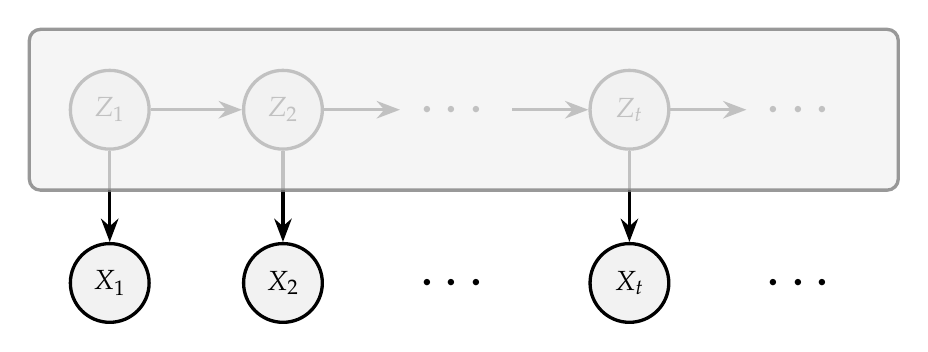
\begin{tikzpicture}[node distance=2.2cm, every state/.style={minimum size=1cm, very thick, fill=gray!10}, auto]

    % States
    \node[state] (Z1) {$Z_1$};
    \node[state] (Z2) [right of=Z1] {$Z_2$};
    \node (dots) [right of=Z2, scale=2] {$\dots$};  % Increased size of dots
    \node[state] (Zt) [right of=dots] {$Z_t$};
    \node (dots1) [right of=Zt, scale=2] {$\dots$};  % Increased size of dots
    \node[state] (X1) [below of=Z1] {$X_1$};
    \node[state] (X2) [right of=X1] {$X_2$};
    \node (dots2) [right of=X2, scale=2] {$\dots$};  % Increased size of dots
    \node[state] (Xt) [right of=dots2] {$X_t$};
    \node (dots3) [right of=Xt, scale=2] {$\dots$};  % Increased size of dots

    % Transitions outside the box
    \path[->, >={Stealth},very thick] 
    % From state 0 to state 1
    (Z1) edge node {} (Z2)
    (Z2) edge node {} (dots)
    (dots) edge node {} (Zt)
    (Zt) edge node {} (dots1)
    (Z1) edge node {} (X1)
    (Z2) edge node {} (X2)
    (Zt) edge node {} (Xt);

    % Hidden state box with gray and opacity
    \begin{scope}[gray, opacity=0.8] % Set gray and opacity
        \node[draw=gray, very thick, fill=gray!10, rounded corners, fit=(Z1) (Z2) (Zt) (dots1), inner sep=0.5cm] {};
    \end{scope}



\end{tikzpicture}


\end{document}